\documentclass[12pt]{article}
\usepackage[utf8]{inputenc}
\usepackage{geometry}
\usepackage{graphicx}
\usepackage{hyperref}
\usepackage{amsmath}
\usepackage{amsfonts}
\usepackage{listings}
\usepackage{xcolor}
\usepackage{float}
\usepackage{longtable}
\usepackage{array}
\usepackage{tabularx}
\usepackage{booktabs}
\usepackage{caption}
\usepackage{url}
\usepackage{tikz}
\usetikzlibrary{matrix, shapes, arrows, positioning, decorations.pathreplacing}
\usepackage[document]{ragged2e}

% Document geometry
\geometry{a4paper, margin=1in}

\title{Module Interface Specification for Angry Birds Alike}
\author{Author: Hossain, Al Jubair}
\date{March 31, 2024}

\begin{document}

\maketitle

\newpage

\section*{Revision History}
\begin{longtable}{|p{2cm}|p{2cm}|p{10cm}|}
    \hline
    \textbf{Date} & \textbf{Version} & \textbf{Notes} \\
    \hline
    March 5, 2024 & 1.0 & Fixed hyperlinks.\\
    March 13, 2024 & 1.0 & Changed section 5.\\
    \hline
    March 31, 2024 & 1.5 & Adding various changes in sections from 3, 4, 5, and 6, adding module information on Physics engine, UI, Game Logic, Environment variables , graphical examples of the game after implementation \\
    \hline
\end{longtable}

\newpage

\tableofcontents

\newpage

\section{Symbols, Abbreviations, and Acronyms}
\begin{longtable}{|l|l|}
    \hline
    \textbf{Symbol/Abbreviation/Acronym} & \textbf{Definition} \\
    \hline
    MIS & Module Interface Specification \\
    SRS & Software Requirements Specification \\
    VnV & Verification and Validation \\
    \hline
\end{longtable}
\section{Introduction}
This document provides the Module Interface Specifications (MIS) for the "Angry Birds Alike" project. It defines the interfaces for each module, detailing their inputs, outputs, and functionality. This MIS is intended to guide the implementation phase, ensuring that module interactions are clear and consistent. Complementary documents include the System Requirement Specifications (SRS), the Verification and Validation (VnV) plan, and the Module Guide (MG).

\section{Notation}
The notation used in this document follows a standardized format for specifying module interfaces:
- \textbf{Data Types}: Descriptions of the data types used within the modules.
- \textbf{Functions}: Specification of module functions, including inputs, outputs, and side effects.
- \textbf{Constants}: Constants used within the modules.
- \textbf{State Variables}: Variables that store the state of the module.

Data Type Notation:
- \textit{integer}: Represented as \textbf{int}, a whole number.
- \textit{real}: Represented as \textbf{float}, a floating-point number.
- \textit{string}: A sequence of characters.

\section{Module Decomposition}
The modules in "Angry Birds Alike" are decomposed according to the hierarchy established in the Module Guide. This decomposition supports the project's architectural design and clarifies the responsibilities of each module.

\subsection{Overview of Modules}
- \textbf{M1 Game Logic Module}: Handles the core gameplay mechanics.
- \textbf{M2 Physics Engine Module}: Manages physics simulations.
- \textbf{M3 User Interface Module}: Controls the game's user interface and input processing.
- \textbf{M4 Graphics Rendering Module}: Responsible for rendering game graphics.
- \textbf{M5 Sound Module}: Manages game audio.

Each module's interface specification is detailed in the following sections.
\section{MIS of Game Logic Module}

This section details the interface for the Game Logic Module, which is central to managing the game's rules, level progression, and scoring.

\subsection{Module}

\textbf{Short Name}: GameLogic

\subsection{Uses}

- Physics Engine Module (for physics calculations)
- User Interface Module (for receiving player actions)

\subsection{Syntax}

\subsubsection{Exported Constants}

None

\subsubsection{Exported Access Programs}

\begin{tabular}{|l|l|l|l|}
\hline
\textbf{Name} & \textbf{In} & \textbf{Out} & \textbf{Exceptions} \\
\hline
initializeLevel & LevelID & -- & LevelNotFound \\
\hline
getScore & -- & integer & -- \\
\hline
launchProjectile & Velocity, Angle & -- & InvalidInput \\
\hline
resetLevel & -- & -- & -- \\
\hline
endGame & -- & -- & -- \\
\hline
\end{tabular}

\subsection{Semantics}

\subsubsection{State Variables}

- currentLevel: LevelID
- score: integer

\subsubsection{Environment Variables}

None

\subsubsection{Assumptions}

- initializeLevel is called before any other access programs to set up the game environment.
- The game's levels are pre-defined and correspond to valid LevelID inputs.

\subsubsection{Access Routine Semantics}

\textbf{initializeLevel(LevelID)}:
- transition: Loads the specified level, setting currentLevel to the given LevelID.
- exception: LevelNotFound if the specified LevelID does not correspond to a defined level.

\textbf{getScore()}:
- output: Returns the current score of the game.

\textbf{launchProjectile(Velocity, Angle)}:
- transition: Launches a projectile with the specified velocity and angle. Updates game state based on the physics simulation.
- exception: InvalidInput if the given Velocity or Angle are out of acceptable ranges.

\textbf{resetLevel()}:
- transition: Resets the current level to its initial state.

\textbf{endGame()}:
- transition: Terminates the current game session.

\subsubsection{Local Functions}

None
\section{MIS of Physics Engine Module}

This section outlines the interface for the Physics Engine Module, responsible for calculating and simulating the physical interactions within the game.

\subsection{Module}

\textbf{Short Name}: PhysicsEngine

\subsection{Uses}

- Game Logic Module (to receive commands related to game actions)

\subsection{Syntax}

\subsubsection{Exported Constants}

None

\subsubsection{Exported Access Programs}

\begin{tabular}{|l|l|l|l|}
\hline
\textbf{Name} & \textbf{In} & \textbf{Out} & \textbf{Exceptions} \\
\hline
calculateTrajectory & Velocity, Angle & Sequence of Points & InvalidInput \\
\hline
detectCollision & Sequence of Points, Objects & Boolean, ImpactPoint & -- \\
\hline
applyPhysicsEffects & ImpactPoint, Objects & -- & -- \\
\hline
\end{tabular}

\subsection{Semantics}

\subsubsection{State Variables}

None

\subsubsection{Environment Variables}

None

\subsubsection{Assumptions}

- The physics engine is initialized and configured before any game levels are loaded or any projectiles are launched.

\subsubsection{Access Routine Semantics}

\textbf{calculateTrajectory(Velocity, Angle)}:
- output: Returns a sequence of points representing the trajectory of a projectile launched with the specified velocity and angle, considering gravitational forces.
- exception: InvalidInput if the given Velocity or Angle are out of acceptable ranges.

\textbf{detectCollision(Sequence of Points, Objects)}:
- output: Returns a boolean indicating whether a collision occurs along the projectile's path, and if so, returns the point of impact (ImpactPoint).
- transition: Checks the trajectory against the position of objects in the game to determine collisions.

\textbf{applyPhysicsEffects(ImpactPoint, Objects)}:
- transition: Applies physics effects (e.g., force, momentum transfer) to objects involved in a collision at the given ImpactPoint.

\subsubsection{Local Functions}

None
\section{MIS of User Interface Module}

This section describes the interface for the User Interface Module, which manages interactions between the player and the game, ensuring a seamless and intuitive gaming experience.

\subsection{Module}

\textbf{Short Name}: UserInterface

\subsection{Uses}

- Physics Engine Module (to initiate projectile motion based on player input)
- Game Logic Module (to update the game state based on player actions)

\subsection{Syntax}

\subsubsection{Exported Constants}

None

\subsubsection{Exported Access Programs}

\begin{tabular}{|l|l|l|l|}
\hline
\textbf{Name} & \textbf{In} & \textbf{Out} & \textbf{Exceptions} \\
\hline
processInput & UserAction & -- & InvalidAction \\
\hline
updateDisplay & GameState & -- & -- \\
\hline
\end{tabular}

\subsection{Semantics}

\subsubsection{State Variables}

None

\subsubsection{Environment Variables}

\textbf{keyboard}: the device from which user input is received

\textbf{display}: the device on which the game state is visually rendered

\subsubsection{Assumptions}

- The user interface is refreshed at regular intervals to reflect the current game state accurately.
- User input is captured continuously during gameplay.

\subsubsection{Access Routine Semantics}

\textbf{processInput(UserAction)}:
- transition: Interprets user actions (e.g., keyboard presses for moving the slingshot, launching the bird) and communicates these actions to the Game Logic Module for processing.
- exception: InvalidAction if the user performs an action that is not recognized or not applicable in the current game state.

\textbf{updateDisplay(GameState)}:
- transition: Updates the visual display based on the current state of the game, including the position of objects, scores, and any other relevant gameplay information.

\subsubsection{Local Functions}

None

\section{Simulation Interface}
The Simulation Interface provides a visual representation of the projectile motion based on user inputs. The following figures show the simulation at different stages of a projectile's flight path.

% Assuming the images are at the path /mnt/data/ and are named appropriately
\subsection{Annotated Initial Launch}
\begin{figure}[H]
\centering
\begin{tikzpicture}
    \node[anchor=south west,inner sep=0] (image) at (0,0) {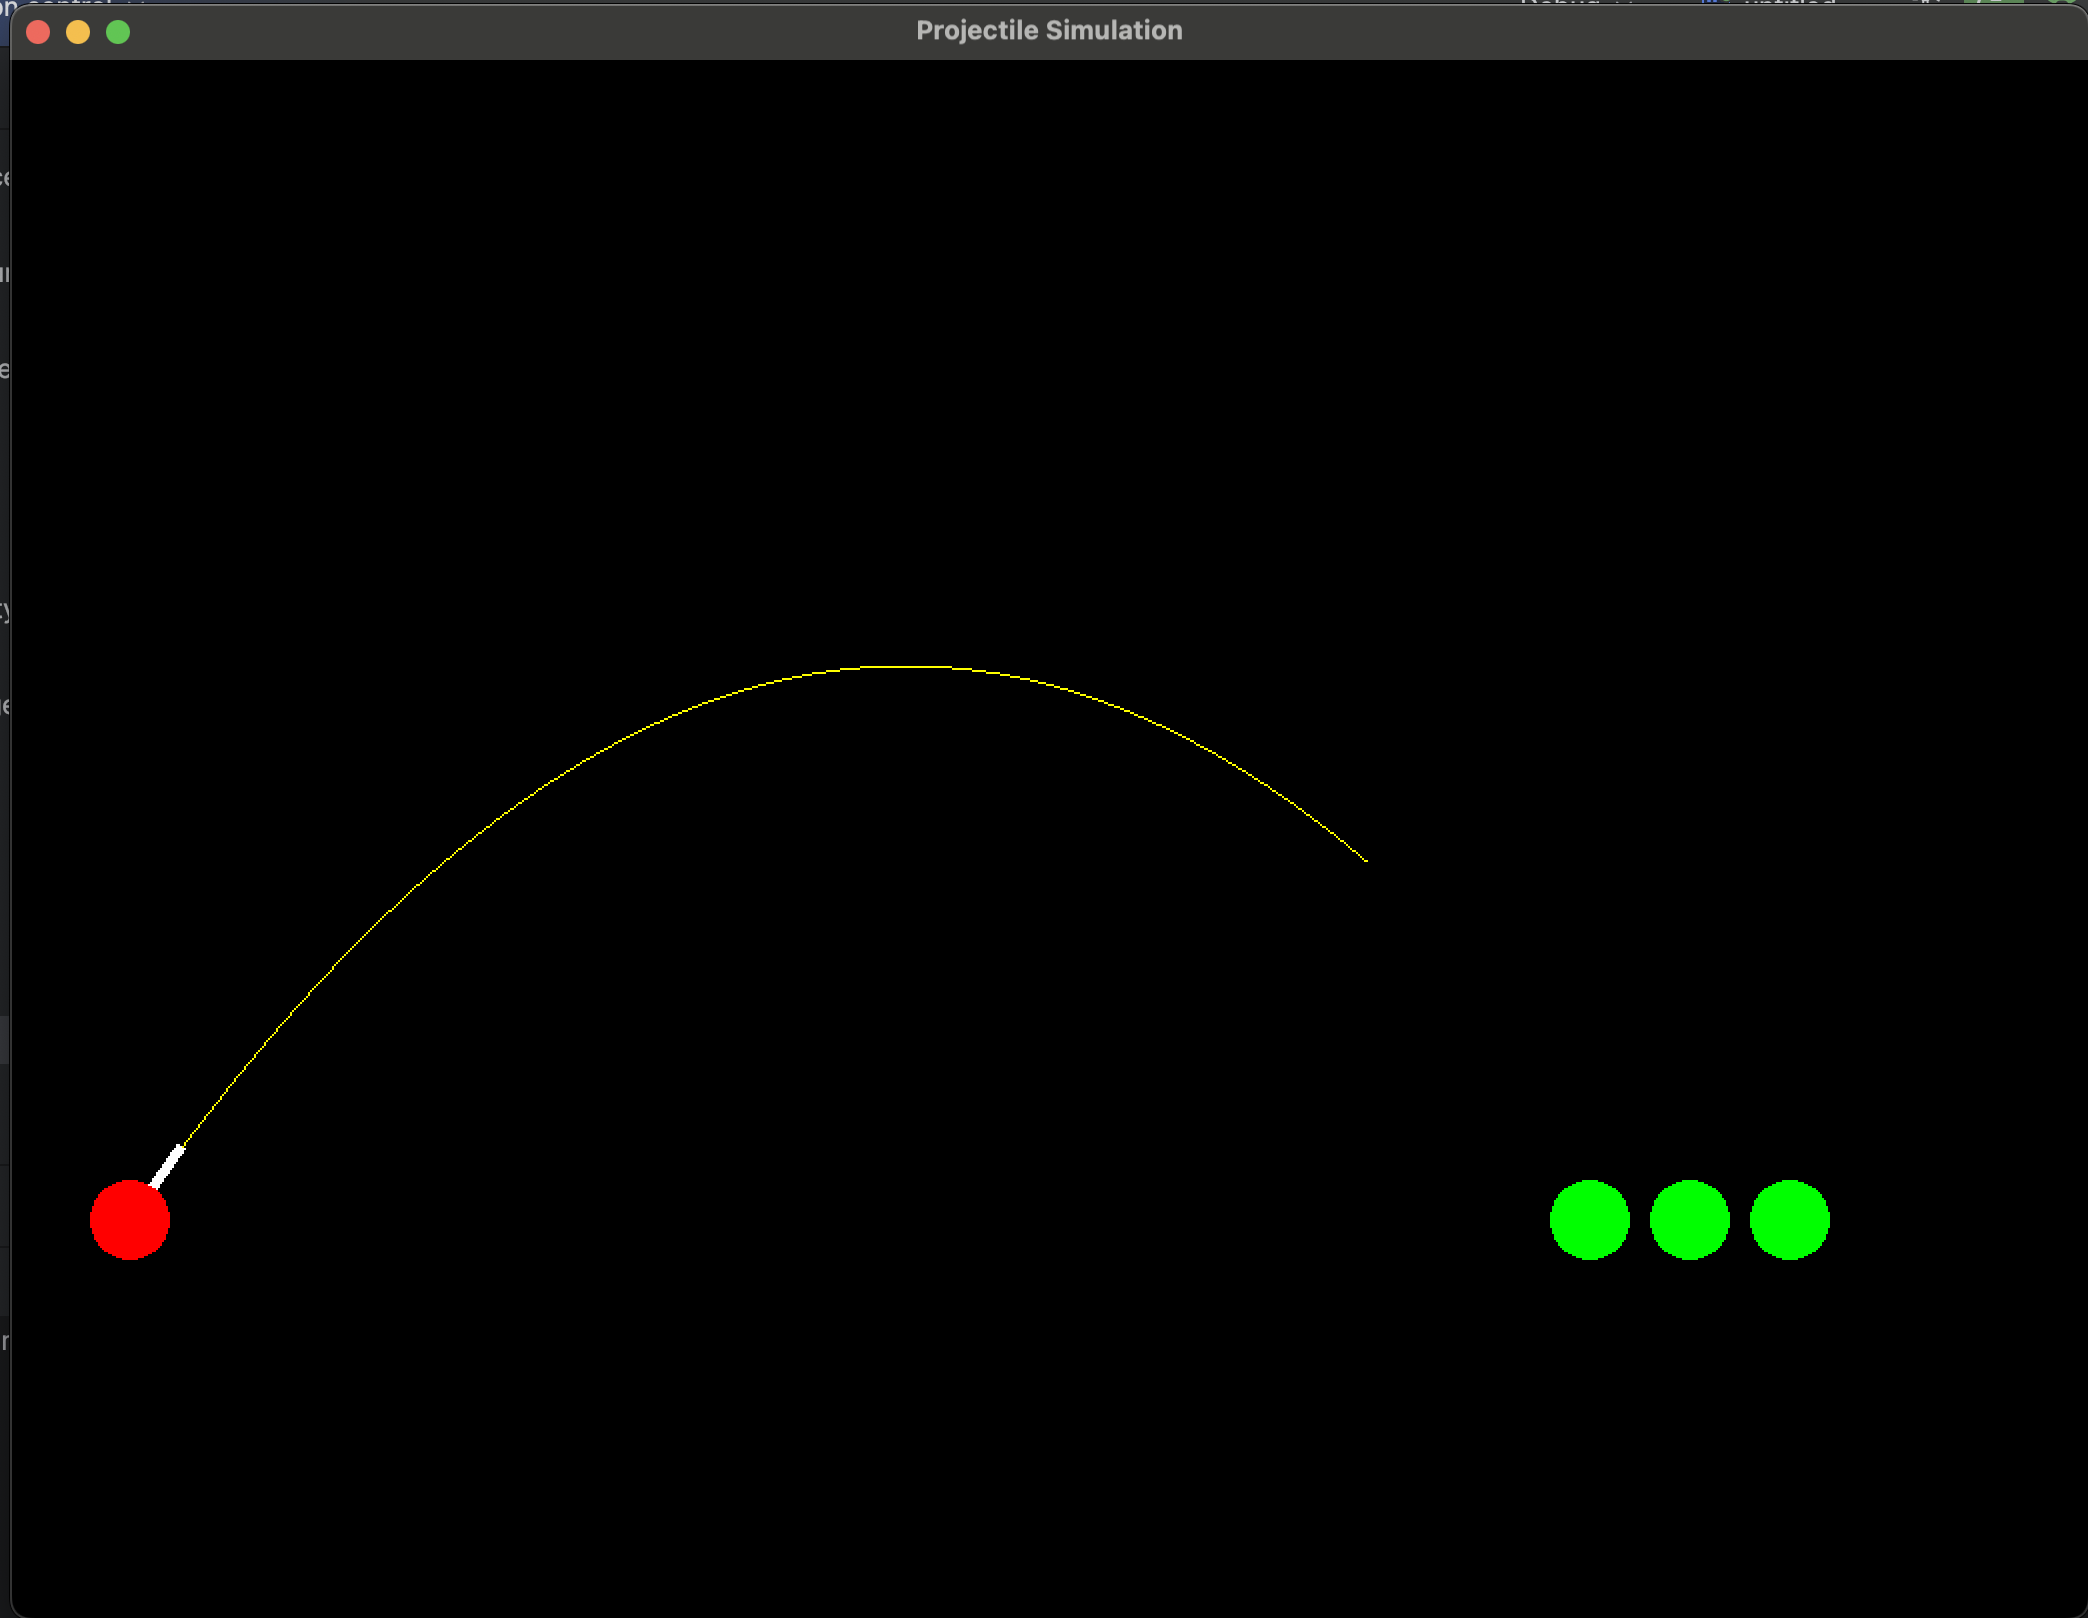
\includegraphics[width=\textwidth]{initi.png}};
    \begin{scope}[x={(image.south east)},y={(image.north west)}]
        % Annotations
        \draw[latex-,thick,red] (0.5,0.7) -- ++(0.1,0.1) node[above right, black, fill=white] {Projectile Path};
        \draw[-latex,thick,blue] (0.1,0.1) -- ++(0.2,0) node[below, black, fill=white] {Launch Direction};
        % Add more annotations as needed
    \end{scope}
\end{tikzpicture}
\caption{Annotated image of the initial stage of the projectile launch.}
\label{fig:annotated_initial_launch}
\end{figure}


\subsection{After Collision}
\begin{figure}[H]
\centering
\begin{tikzpicture}
    \node[anchor=south west,inner sep=0] (image) at (0,0) {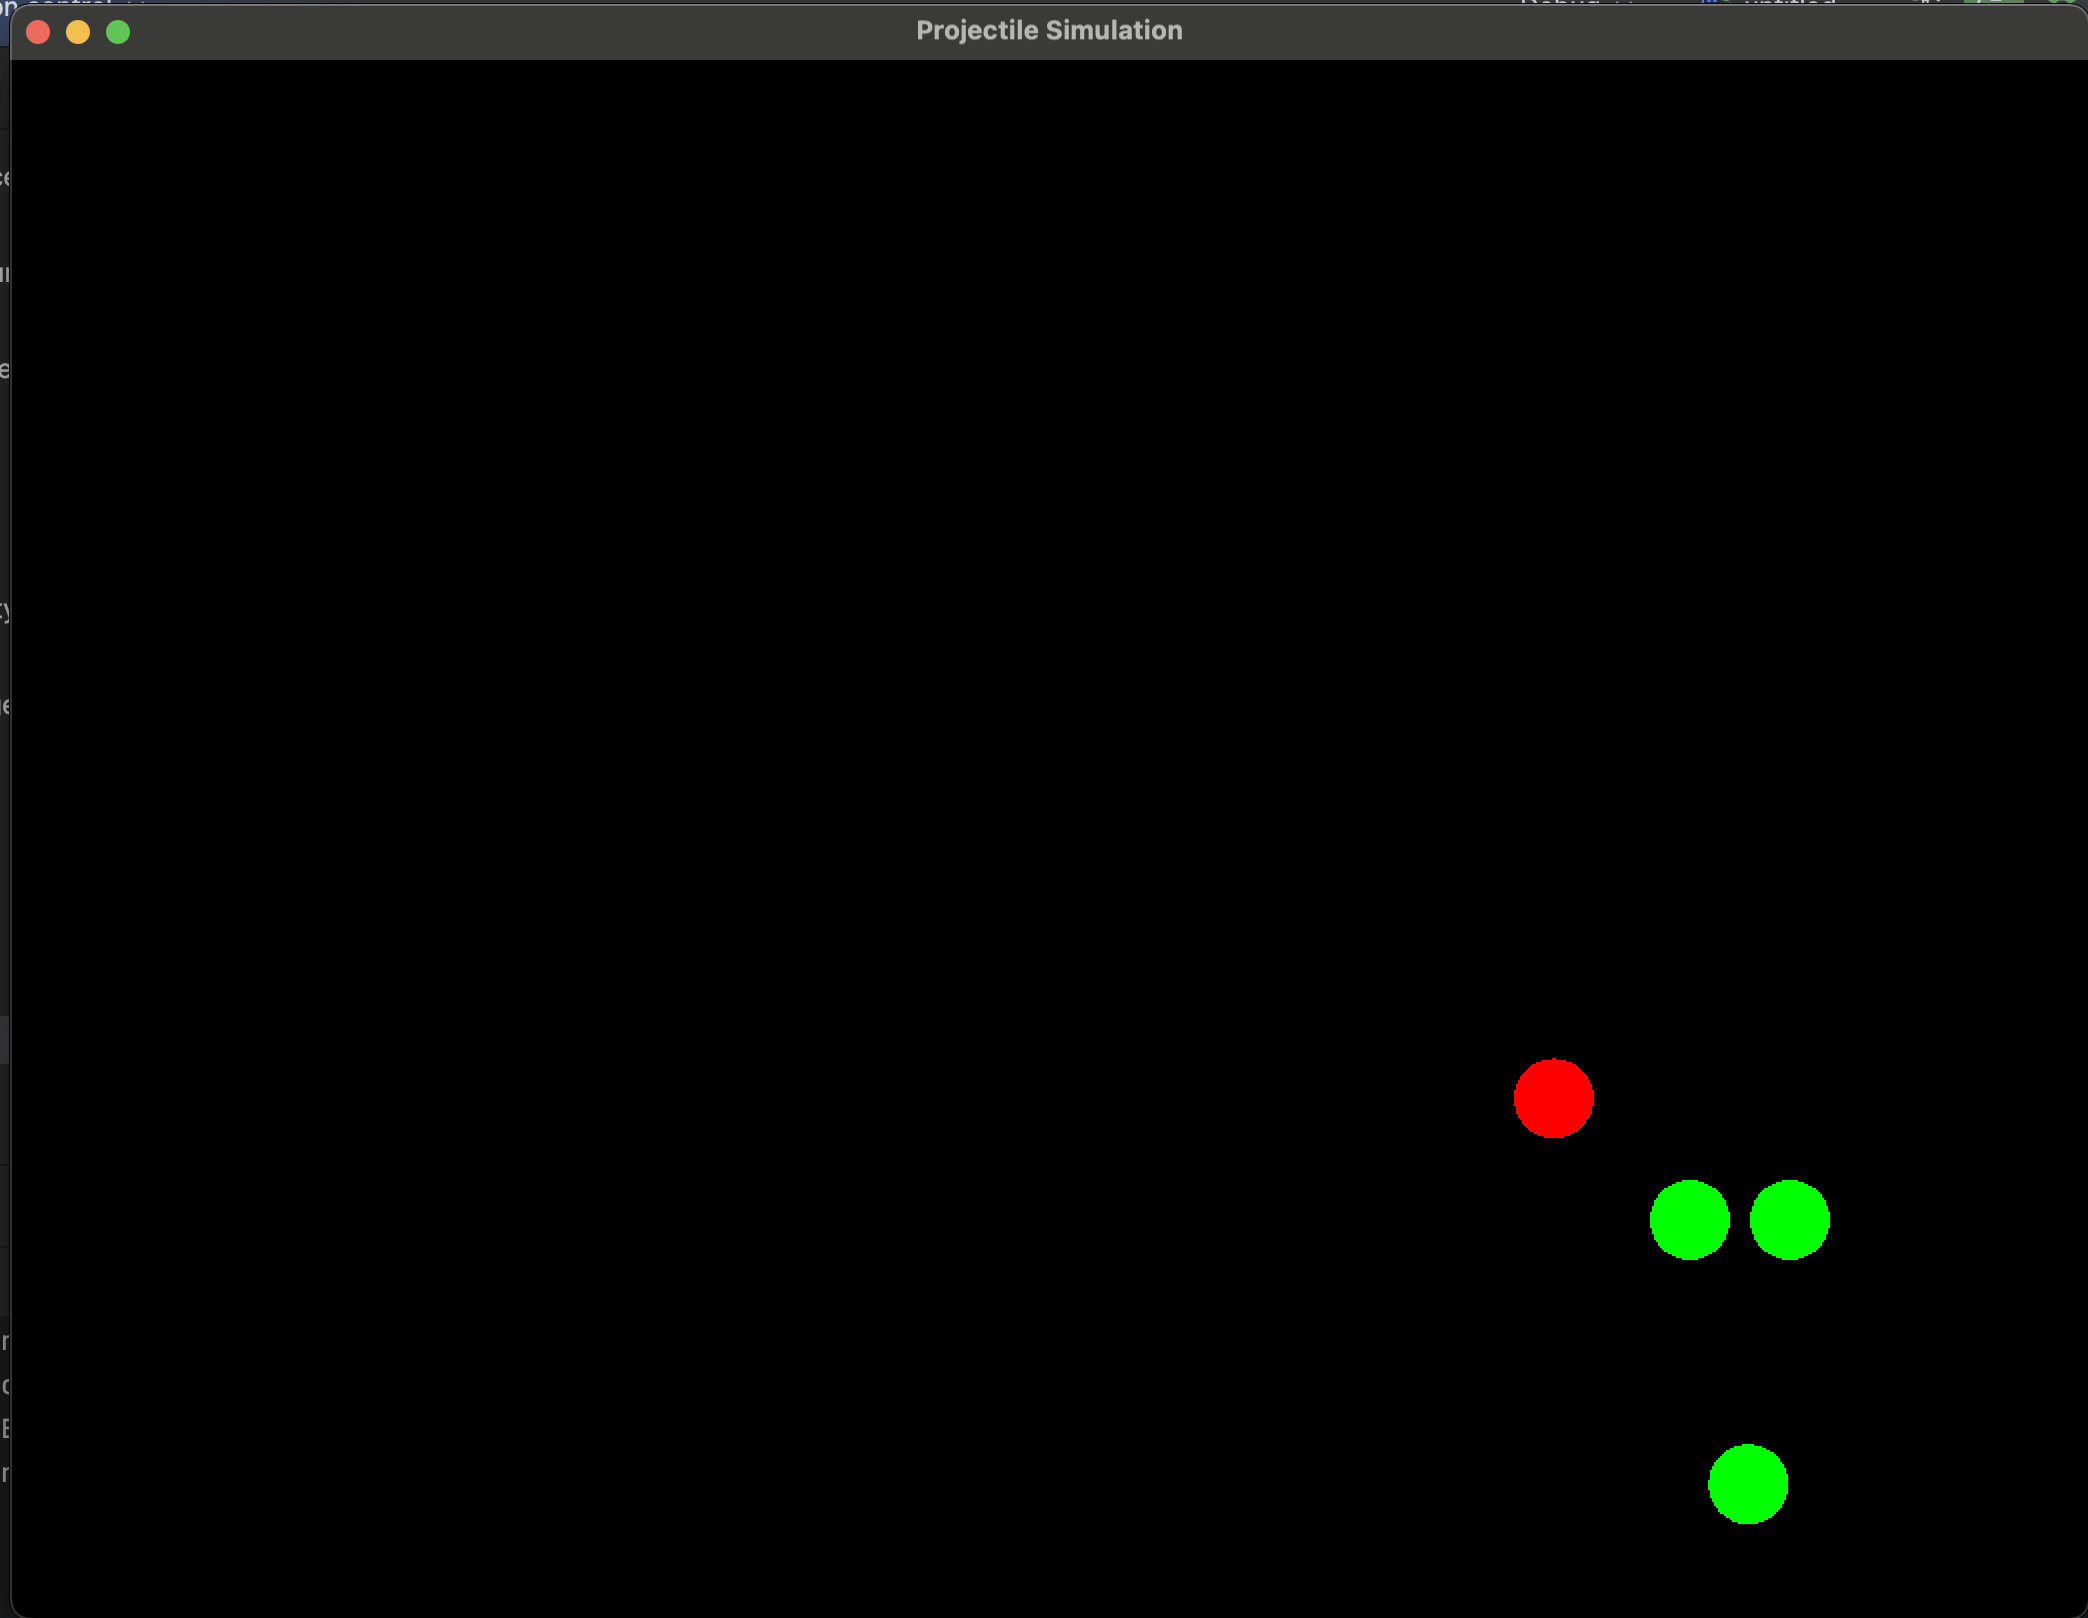
\includegraphics[width=\textwidth]{afterc.png}};
    \begin{scope}[x={(image.south east)},y={(image.north west)}]
        % Annotations
        \draw[latex-,thick,red] (0.8,0.5) -- ++(0.1,0.2) node[above right, black, fill=white] {Post-collision Path};
        \draw[latex-,thick,green] (0.8,0.2) -- ++(0.1,-0.1) node[below right, black, fill=white] {Debris Trajectory};
        \draw[fill=red,red] (0.75,0.2) circle (3pt) node[above left, black, fill=white] {Collision Point};
        % Add more annotations as needed
    \end{scope}
\end{tikzpicture}
\caption{Projectile in mid-flight, after colliding with targets.}
\label{fig:after_collision}
\end{figure}


\section{MIS of Game Logic Module}

This section outlines the interface for the Game Logic Module. This module is essential for controlling the flow of the game, managing levels, player scores, and enforcing the game rules.

\subsection{Module}

\textbf{Short Name}: GameLogic

\subsection{Uses}

- Physics Engine Module (to simulate physical interactions)
- User Interface Module (to receive player inputs)

\subsection{Syntax}

\subsubsection{Exported Constants}

None

\subsubsection{Exported Access Programs}

\begin{tabular}{|l|l|l|l|}
\hline
\textbf{Name} & \textbf{In} & \textbf{Out} & \textbf{Exceptions} \\
\hline
startLevel & LevelID & -- & InvalidLevelException \\
\hline
endLevel & -- & LevelOutcome & -- \\
\hline
updateScore & ScoreUpdate & -- & -- \\
\hline
resetLevel & -- & -- & -- \\
\hline
\end{tabular}

\subsection{Semantics}

\subsubsection{State Variables}

- currentLevel: LevelID
- currentScore: integer

\subsubsection{Environment Variables}

None

\subsubsection{Assumptions}

- startLevel is called at the beginning of each level.
- endLevel is called when a level is completed or the player fails.

\subsubsection{Access Routine Semantics}

\textbf{startLevel(LevelID)}:
- transition: Initializes the game state for the specified level. This includes setting up the initial positions of objects, resetting the score for the level, and preparing the physics engine for simulation.
- exception: InvalidLevelException is thrown if the LevelID does not correspond to a valid level.

\textbf{endLevel()}:
- output: Returns an outcome of the current level, indicating whether the player has succeeded or failed, and any rewards earned. The game state is updated accordingly.
- exception: None

\textbf{updateScore(ScoreUpdate)}:
- transition: Adjusts the current score based on actions taken during the level, such as destroying targets or completing objectives.
- exception: None

\textbf{resetLevel()}:
- transition: Resets the current level to its initial state, including reinitializing the positions of objects and resetting the score.
- exception: None

\subsubsection{Local Functions}

None
\section{MIS of User Interface Module}

This section provides details on the User Interface Module, which is responsible for handling all player interactions and updating the game display accordingly.

\subsection{Module}

\textbf{Short Name}: UserInterface

\subsection{Uses}

- Game Logic Module (to communicate player actions and receive game state updates)
- Physics Engine Module (for displaying physics-based animations)

\subsection{Syntax}

\subsubsection{Exported Constants}

None

\subsubsection{Exported Access Programs}

\begin{tabular}{|l|l|l|l|}
\hline
\textbf{Name} & \textbf{In} & \textbf{Out} & \textbf{Exceptions} \\
\hline
displayMainMenu & -- & -- & -- \\
\hline
displayLevel & LevelID & -- & InvalidLevelException \\
\hline
getPlayerInput & -- & PlayerAction & -- \\
\hline
updateDisplay & GameState & -- & -- \\
\hline
\end{tabular}

\subsection{Semantics}

\subsubsection{State Variables}

- currentScreen: ScreenType

\subsubsection{Environment Variables}

- screen: a display device

\subsubsection{Assumptions}

- The UI module is initialized before any player interaction.
- The display device is capable of rendering the game's graphics.

\subsubsection{Access Routine Semantics}

\textbf{displayMainMenu()}:
- transition: Changes the currentScreen to the main menu and updates the display device to show the main menu options.
- exception: None

\textbf{displayLevel(LevelID)}:
- transition: Loads the specified level's visual elements and prepares the screen for gameplay.
- exception: InvalidLevelException is thrown if the LevelID does not correspond to a valid level.

\textbf{getPlayerInput()}:
- output: Captures and returns the player's input as a PlayerAction, which includes moving the launcher, firing a projectile, or navigating the UI.
- exception: None

\textbf{updateDisplay(GameState)}:
- transition: Updates the game's visual representation on the display device based on the current game state, including the positions of objects, scores, and any UI elements.
- exception: None

\subsubsection{Local Functions}

None

\newpage
\section{Appendix}

\subsection{Physics Equations and Concepts}

This appendix provides a brief overview of the physics equations and concepts utilized within the Physics Engine Module to simulate realistic interactions within the game.

\subsubsection*{Projectile Motion}

The trajectory of a projectile is calculated using the initial velocity (\(v_0\)), the angle of launch (\(\theta\)), and the acceleration due to gravity (\(g\)). The horizontal (\(x\)) and vertical (\(y\)) positions at any time \(t\) can be calculated as follows:

- Horizontal position: \( x(t) = v_{0x} \cdot t \)
- Vertical position: \( y(t) = v_{0y} \cdot t - \frac{1}{2} g t^2 \)

where \( v_{0x} = v_0 \cdot \cos(\theta) \) and \( v_{0y} = v_0 \cdot \sin(\theta) \).

\subsubsection*{Collision Detection and Response}

The module employs basic principles of momentum and energy conservation to simulate collisions between objects. When two objects collide, the module calculates the new velocities based on the masses and initial velocities of the objects involved.

\subsubsection*{Gravity and Other Forces}

Gravity is a constant force acting downward on all objects. The module also accounts for other forces, such as applied forces when a bird is launched, to update the velocities and positions of objects.

\subsection{Glossary of Terms}

- \textbf{Projectile}: An object thrown into space upon which the only force acting is gravity.
- \textbf{Trajectory}: The path followed by a projectile flying or an object moving under the action of given forces.
- \textbf{Collision}: An event where two or more bodies exert forces on each other in a relatively short time.
- \textbf{Gravity}: A force that attracts a body towards the center of the earth, or towards any other physical body having mass.

\newpage
\section{Reflection}

The development of "Angry Birds Alike" has been a comprehensive exercise in applying theoretical knowledge to a practical, engaging project. This section reflects on various aspects of the project's development, highlighting challenges encountered, solutions devised, and learning outcomes.

\subsection{Challenges and Solutions}

One of the most significant challenges was accurately simulating the physics involved in the game. Implementing a realistic trajectory calculation for the birds required a deep understanding of projectile motion physics and the application of numerical methods for solving differential equations. To address this, extensive research into physics simulation techniques was undertaken, and the Runge-Kutta method (RK4) was implemented for its balance between accuracy and computational efficiency.

Another challenge I think, will be designing a user interface that is intuitive yet provides all necessary controls for the game. Achieving this required iterative design and testing, incorporating feedback from trial users to refine the UI/UX until it met the desired standards of accessibility and engagement.

\subsection{Key Learning Outcomes}

\textbf{Problem-Solving Skills:} Developing this game honed my ability to break down complex problems into manageable components, apply theoretical knowledge to practical situations, and devise effective solutions.

\textbf{Software Engineering Principles:} This project reinforced the importance of modular design, information hiding, and the use of design patterns in creating maintainable and scalable software.

\textbf{Physics Simulation:} I gained valuable experience in simulating real-world physics within a digital environment, an area that blends scientific knowledge with creative problem-solving.

\subsection{Future Improvements}

Given more time and resources, I would explore the implementation of more complex physics interactions, such as wind resistance, to add another layer of challenge and realism to the game. Additionally, integrating a more sophisticated AI for the game's opponents could enhance the gameplay, making it more dynamic and unpredictable.

\subsection{Conclusion}

"Angry Birds Alike" has been a challenging yet rewarding project that has significantly contributed to my growth as a software developer and problem-solver. It underscored the importance of a solid theoretical foundation, the value of user-centered design, and the necessity of perseverance through the challenges inherent in software development.

\end{document}